\documentclass[11pt,a4paper]{article}
\usepackage[utf8]{inputenc}
\usepackage[T1]{fontenc}
\usepackage{amsfonts}
\usepackage{amssymb}
\usepackage{mdframed}
\usepackage{tikz}
\usepackage{tkz-tab}
\usepackage{pgfplots}
\usepackage{pgfkeys}
\usepackage{xcolor}
\usepackage{fancyhdr}
\usepackage{lastpage}
\usepackage[fleqn]{amsmath}
\setlength{\mathindent}{0pt}

% Spécifications du document
\newcommand{\doctitre}{Fonction exponentielle et logarithme népérien} % Ex: Le second degré
\newcommand{\docniveau}{$1^{\text{re}}$ Spécialité mathématiques} % Ex: $1^{\text{re}}$ Spécialité mathématiques
\newcommand{\doctheme}{Analyse} %Ex: Algèbre
\newcommand{\doctype}{Cours} % Ex: Démonstrations
\newcommand{\docshorttype}{Cours} % Démo

% Couleurs pour les graphiques
\definecolor{dark_green}{HTML}{008000}

% Paramètres du document
\RequirePackage{geometry}
\geometry{tmargin=1cm,bmargin=1.9cm,lmargin=1.9cm,rmargin=1.9cm}
% \renewcommand{\familydefault}{\sfdefault}
\setlength{\parindent}{0pt}
\title{\doctitre}
\author{\docniveau \\ \doctheme\text{ - }\doctype}
\date{}
\fancypagestyle{custom}{
  \fancyhf{}
  \renewcommand{\headrulewidth}{0pt}
  \lfoot{\doctheme\text{ - }\docshorttype}
  \cfoot{\doctitre} % Change \titre to \doctitre
  \rfoot{\thepage/\pageref{LastPage}}
}

% Styles pour les mdframed
\mdfdefinestyle{definitionStyle}{
    leftline=true,
    rightline=false,
    topline=false,
    bottomline=false,
    linewidth=2pt,
    linecolor=black,
    innertopmargin=0pt,
    innerbottommargin=0pt,
    innerrightmargin=0pt,
    innerleftmargin=5pt,
}

\mdfdefinestyle{proprieteStyle}{
    linewidth=1pt,
    linecolor=black,
    innertopmargin=5pt,
    innerbottommargin=5pt,
    innerrightmargin=5pt,
    innerleftmargin=5pt,
}
% ----- DEBUT DU DOCUMENT -----
\begin{document}

% Style et numérotation
\maketitle
\pagestyle{custom}
\thispagestyle{custom}

\section{Généralités sur la fonction exponentielle}

\begin{mdframed}[style=definitionStyle]
    \textbf{Définition et propriété admise :} ~\\
    Il existe une unique fonction $f$ dérivable sur $\mathbb{R}$ telle que $f'=f$ et $f(0)=1$. \\
    Cette fonction est appelée fonction exponentielle et se note $\exp$. \\
    Ainsi, pour tout réel $x$, on a $\exp'(x)=\exp(x)$ et $\exp(0)=1$.
\end{mdframed}

\subsection{Propriétés algébriques}

\begin{mdframed}[style=proprieteStyle]
    \textbf{Lemme :} ~\\
    Pour tout réel $x$, on a $\exp(x)\not=0$.
\end{mdframed}

\begin{mdframed}[style=proprieteStyle]
    \textbf{Propriétés :}
    \begin{enumerate}
        \item Pour tous réels $x$ et $y$, on a $\exp(x+y)=\exp(x)\times\exp(y)$ qu'on appelle relation fonctionnelle.
        \item Pour tous réels $x$ et $y$, on a :
        \begin{itemize}
            \item $\displaystyle\exp(-x)=\frac{1}{\exp(x)}$
            \item $\displaystyle\exp(x-y)=\frac{\exp(x)}{\exp(y)}$ 
            \item $\displaystyle\exp(nx)=\exp(x)^n$ 
        \end{itemize}
    \end{enumerate}
\end{mdframed}

\subsection{La notation de l'exponentielle}

\begin{mdframed}[style=definitionStyle]
    \textbf{Définition :} ~\\
    L'image de $1$ par la fonction $\exp$ est le nombre noté $e$, appelé constante d'Euler. Ainsi, $\exp(1)=e$.
\end{mdframed}

\textbf{Remarque :} La fonction $\exp$ possède les mêmes propriété algébriques que les fonctions puissances. On notera donc $\exp(x)=e^x$ ($e\approx2,7182\dots$).

\begin{mdframed}[style=proprieteStyle]
    \textbf{Propriété :} ~\\
    Pour tous réels $x$ et $y$, on a : \\

    \begin{minipage}{0.25\textwidth}
        \begin{itemize}
            \item $\displaystyle e^{x+y}=e^x\times e^y \color{white}\frac{e^x}{e^y}$ 
            \item $\displaystyle e^{-x}=\frac{1}{e^x}$
        \end{itemize}
    \end{minipage}
    \hfill
    \begin{minipage}{0.8\textwidth}
        \begin{itemize}
            \item $\displaystyle e^{x-y}=\frac{e^x}{e^y}$ 
            \item $\displaystyle (e^x)^n=e^{nx}\color{white}\frac{e^x}{e^y}$ 
        \end{itemize}
    \end{minipage}
\end{mdframed}

\subsection{Lien avec les suites géométriques}

\begin{mdframed}[style=proprieteStyle]
    \textbf{Propriété :} ~\\
    Soit $a$ un réel. Soit $u$ la suite définie pour tout entier naturel $n$ par $u_n=e^{na}$. \\
    Alors la suite $u$ est une suite géométrique.
\end{mdframed}

\section{Étude et applications de la fonction exponentielle}

\subsection{Signe de la fonction exponentielle}

\begin{mdframed}[style=proprieteStyle]
    \textbf{Propriété :} ~\\
    La fonction $\exp$ est strictement positive sur $\mathbb{R}$. \\
    Autrement dit : pour tout nombre réel $x$, $e^x>0$.
\end{mdframed}

\subsection{Variations de la fonction exponentielle}

\begin{minipage}[t]{0.35\textwidth} % Adjust the width of the first minipage
    $\displaystyle{\color{white}1}$
    \begin{mdframed}[style=proprieteStyle]
        \textbf{Propriété :} ~\\
        La fonction $\exp$ est strictement croissante sur $\mathbb{R}$.
    \end{mdframed}
\end{minipage}
\hspace{0.06\textwidth} % Add horizontal space here
\begin{minipage}[t]{0.6\textwidth} % Adjust the width of the second minipage
    On résume dans le tableau de variation suivant : $\displaystyle{\color{white}\frac{1}{1}}$ ~\\
    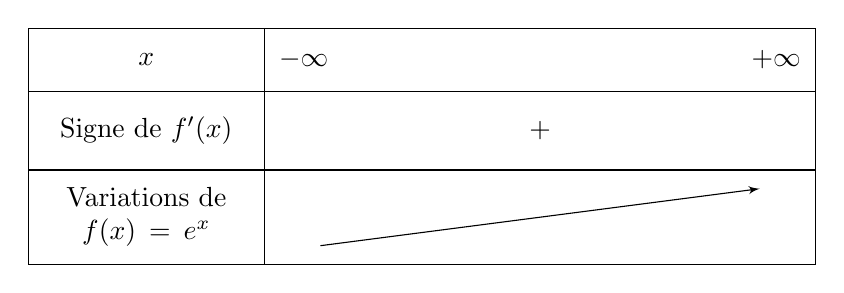
\begin{tikzpicture}
        \tkzTabInit[lgt=3,espcl=6]{$x$ / 0.8 , Signe de $f'(x)$ / 1, Variations de $f(x)=e^x$ / 1.2}{$-\infty$, $+\infty$}
        \tkzTabLine{,+,}
        \tkzTabVar{-/ , +/ }
    \end{tikzpicture}
\end{minipage}



\subsection{Courbe de la fonction exponentielle}

\begin{minipage}{0.2\textwidth}
\begin{tabular}{|c|c|}
    \hline
    $x$ & $e^x$ \\
    \hline
    $-2$ & $\approx0,13$ \\
    \hline
    $-1,5$ & $\approx0,22$ \\
    \hline
    $-1$ & $\approx0,37$ \\
    \hline
    $-0,5$ & $\approx0,61$ \\
    \hline
    $0$ &  $1$ \\
    \hline
    $0,5$ &  $\approx1,65$ \\
    \hline
    $1$ &  $\approx2,72$ \\
    \hline
    $1,5$ &  $\approx4,48$ \\
    \hline
    $2$ & $\approx7,39$ \\
    \hline
\end{tabular}
\end{minipage}
\hfill
\begin{minipage}{0.8\textwidth}
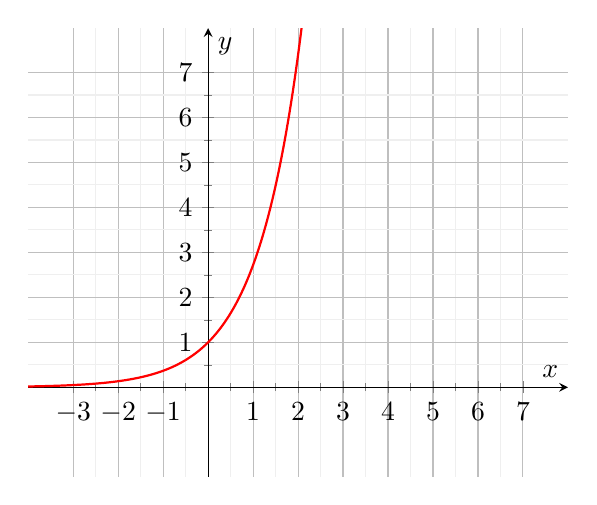
\begin{tikzpicture}
    \begin{axis}[
        axis lines = middle,
        axis equal,
        samples=200,
        xlabel = $x$,
        ylabel = {$y$},
        xmin=-4, xmax=8,
        ymin=-1, ymax=7,
        xtick = {-3, -2,...,7},
        ytick = {0, 1,...,7},
        grid = both,
        minor tick num = 1,
        major grid style = {lightgray},
        minor grid style = {lightgray!25}
    ]
    \addplot[red, thick] {exp(x)};
\end{axis}
\end{tikzpicture}
\end{minipage}

\subsection{Fonctions définies par $f(t)=e^{kt}$ avec $k\in\mathbb{R}$}

\begin{mdframed}[style=proprieteStyle]
    \textbf{Propriété :} ~\\
    Pour $k>0$, la fonction $f$ définie par $f(t)=e^{kt}$ est strictement croissante sur $\mathbb{R}.$ \\
    Pour $k<0$, la fonction $f$ définie par $f(t)=e^{kt}$ est strictement décroissante sur $\mathbb{R}.$ 
\end{mdframed}

\subsection{Fonctions du type $f:x\mapsto e^{ax+b}$}

\begin{mdframed}[style=proprieteStyle]
    \textbf{Propriété :} ~\\
    Pour $a$ et $b$ fixés, la fonction $f$ définie sur $\mathbb{R}$ par $f(x)=e^{ax+b}$ est dérivable sur $\mathbb{R}$ et pour tout réel $x$, $f'(x)=a\times e^{ax+b}$.
\end{mdframed}


\subsection{Équations et inéquations}

\begin{mdframed}[style=proprieteStyle]
    \textbf{Propriété :} ~\\
    Pour tous réels $a$ et $b$, on a :
    \vspace{-4pt}
    \begin{itemize}
        \item $e^a=e^b \Leftrightarrow a=b$
        \item $e^a<e^b \Leftrightarrow a<b$
    \end{itemize}
\end{mdframed}

\newpage

\textbf{Exemples :} ~\\

\begin{minipage}{0.5\textwidth}
    \begin{itemize}
        \item On résout dans $\mathbb{R}$ l'équation $e^{2x+1}=e^{x-3}$ :
        \begin{align*}
            &e^{2x+1}=e^{x-3} \\
            \Leftrightarrow\text{ }&2x+1=x-3 \\
            \Leftrightarrow\text{ }&x+1=-3 \\
            \Leftrightarrow\text{ }&x=-4 \\
            \Leftrightarrow\text{ }&S=\{-4\}
        \end{align*}
    \end{itemize}
\end{minipage}
\hfill
\begin{minipage}{0.5\textwidth}
    \begin{itemize}
        \item On résout dans $\mathbb{R}$ l'inéquation $e^{x-3}<1$ :
        \begin{align*}
            &e^{x-3}<1 \\
            \Leftrightarrow\text{ }&e^{x-3}<e^0 \\
            \Leftrightarrow\text{ }&x-3<0 \\
            \Leftrightarrow\text{ }&x<3 \\
            \Leftrightarrow\text{ }&S=]-\infty;3[
        \end{align*}
    \end{itemize}
\end{minipage}

\section{Généralités sur la fonction logarithme}

\subsection{Introduction}

\begin{mdframed}[style=proprieteStyle]
    \textbf{Théorème :} ~\\
    Pour tout réel $a>0$, il existe un unique réel $b$ tel que $a=e^b$.
\end{mdframed}

\subsection{Définition et notation}

\begin{mdframed}[style=definitionStyle]
    \textbf{Définition :} ~\\
    On appelle logarithme népérien d'un réel $a>0$, le nombre réel $b$ tel que $e^b=a$.\\
    On le note $\ln(a)=b$. 
\end{mdframed}

\textbf{Exemple :}
\vspace{-4pt}
\begin{itemize}
    \item $\ln(1) = 0$ (car $e^0=1$)
    \item $\ln(e) = 1$ (car $e^1=e$)
\end{itemize}

\textbf{Remarques :}
\vspace{-4pt}
\begin{itemize}
    \item $\ln(0)$ n'existe pas. En effet, $e^x\not=0$ pour tout $x\in\mathbb{R}$
    \item Pour tout entier $n\geq 2$, $\ln(n)$ n'est pas rationel.
\end{itemize} 

\subsection{Propriétés algébriques}

\begin{mdframed}[style=proprieteStyle]
    \textbf{Théorème :} ~\\
    Pour tout réel $x>0$, $y>0$ et pour tout entier relatif $n$,
    \vspace{-4pt}
    \begin{itemize}
        \item $e^{\ln(x)}=x$
        \item $\ln(e^x)=x$
        \item $\ln(xy) = \ln(x) + \ln(y)$
        \item $\ln(\frac{x}{y}) = \ln(x) - \ln(y)$
        \item $\ln(x^n)=n\ln(x)$
    \end{itemize}
\end{mdframed}

\section{Propriétés graphiques}

\subsection{Symétrie des courbes représentatives de l'exponentielle et du logarithme}

\begin{minipage}{0.5\textwidth}
    Dans un repère orthonormé, on note $d$ la droite d'équation $x=y$.\\
La symétrie axiale par rapport à la droite $d$ a pour effet d'échanger les abscisses et les ordonnées, c'est à dire
qu'elle transforme tout point de coordonnées $(x;y)$ en un point de coordonnées $(x;y)$. \\

\begin{mdframed}[style=proprieteStyle]
    \textbf{Théorème :} ~\\
    Les courbes représentatives de la fonction $\exp$ et $\ln$ sont symétriques l'une de l'autre par rapport à la droite $d$.
\end{mdframed}
\end{minipage}
\hfill
\begin{minipage}{0.4\textwidth}
    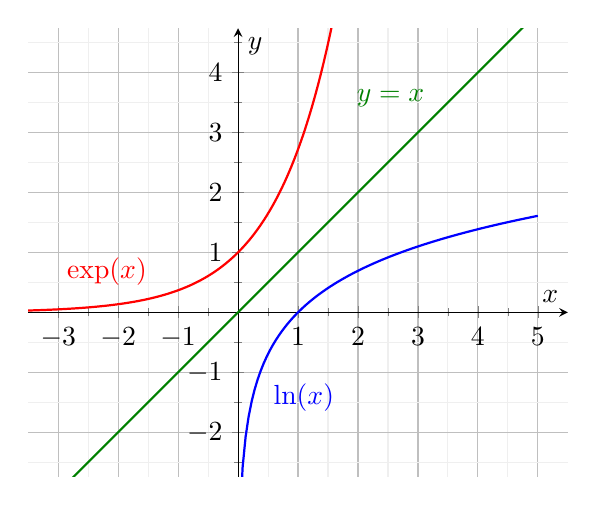
\begin{tikzpicture}
        \begin{axis}[
            axis lines = middle,
            axis equal,
            samples=200,
            xlabel = $x$,
            ylabel = {$y$},
            xmin=-3.5, xmax=5.5,
            ymin=-2, ymax=4,
            xtick = {-3, -2,...,5},
            ytick = {-3, -2,...,5},
            grid = both,
            minor tick num = 1,
            major grid style = {lightgray},
            minor grid style = {lightgray!25}
        ]
        \addplot[red, thick] {exp(x)};
        \addplot[blue, thick] {ln(x)};
        \addplot[dark_green, thick] {x};
    \end{axis}
    \node at (1,2.6) {$\color{red}\exp(x)$};
    \node at (4.6,4.8) {$\color{dark_green}y=x$};
    \node at (3.5,1) {$\color{blue}\ln(x)$};
    \end{tikzpicture}
\end{minipage}

\subsection{Dérivation de la fonction logarithme}

\begin{mdframed}[style=proprieteStyle]
    \textbf{Théorème :} ~\\
    Si pour tout réel $x>0$, $f(x)=\ln(x)$ alors $f$ est dérivable, et pour tout $x>0$ : $\displaystyle f'(x)=\frac{1}{x}$
\end{mdframed}

\begin{mdframed}[style=proprieteStyle]
    \textbf{Corrolaire :}
    \begin{itemize}
        \vspace{-4pt}
        \item La fonction $\ln(x)$ est strictement croissante sur $]0;+\infty[$.
        \item Pour tous réels $a$ et $b$ strictements positifs, $\ln(a)<\ln(b)\Leftrightarrow a<b$.
    \end{itemize}
\end{mdframed}

\end{document}
% ----- FIN DU DOCUMENT -----